\section{Decay-Candidate Selection and Background}
\label{sec:ana_bkgSub}

Whereas the decay model discussed in Chapter~\ref{chap:pheno} describes the time and angular distribution of \BstoJpsiKK{} signal decays,
the experimental data contains both signal and background decay candidates. The background distribution is subtracted from the total
distribution in the data to be able to fit the model to the distribution of signal decays. Since there are statistical uncertainties
associated to both the total distribution and the subtracted background distribution, the resulting uncertainties in the signal-parameter
estimates become larger with an increasing amount of background decay candidates. Therefore, a selection procedure is applied, designed to
reject as many background candidates as possible without removing too many signal candidates.


%%%%%%%%%%%%%%%%%%%%%%%%%%%%%
\subsection{Selection}
\label{subsec:ana_bkgSub_sel}
%%%%%%%%%%%%%%%%%%%%%%%%%%%%%

The decay-candidate selection procedure was introduced in Section~\ref{subsec:intro_LHCb_Jpsiphi} and is briefly described in the context
of the \BstoJpsiKK{} decay here. See reference~\cite{Aaij:2015} for a detailed discussion.

As described in Section~\ref{subsec:intro_LHCb_Jpsiphi}, the first selection requirements are applied in the L0 trigger, which only selects
events with hits in the muon stations and particles with a sufficiently high (transverse) momentum. From the events that remain, the HLT
reconstructs and selects $\mumu$ pairs that are likely to originate from a $\Jpsi\to\mumu$ decay. Offline, the resulting $\Jpsi\to\mumu$
candidates are matched to $\KK$ pairs to form \BstoJpsiKK{} decay candidates. The four tracks these candidates consist of are required to
be compatible with a $\Bs$ that was produced in the associated primary vertex and decayed at a decay time above a given threshold.

In both HLT1 and HLT2 there are two different types of selections applied. The first type does not use any information on the distance that
the $\Bs$ travelled before it decayed and the second type does. Requiring a minimum flight distance reduces the fraction of
background candidates significantly, since all four tracks originate from the primary vertex for most combinatorial background, while the
tracks in a $\Bs$ decay originate from a secondary vertex at some distance from the primary vertex. However, the flight distance variable
is correlated with the decay time variable and requiring a minimum flight distance introduces a non-trivial selection efficiency as a
function of decay time. Therefore, the sets of selection criteria that use information on the flight distance are called \emph{decay-time
biasing} or \emph{biased}.

The unbiased HLT1 selection requires two oppositely charged muon candidates that are close enough to originate from one decay vertex and
have a $\mumu$ invariant mass greater than 2.7\unitsp\GeV. The biased HLT1 selection does not require a $\Jpsi$ candidate, but selects
single tracks with a perpendicular distance to any primary vertex greater than 0.1\unitsp{}mm. Both of these selections reduce the number
of selected events to a manageable level. Approximately 68\% of the decay candidates that are finally used in the fit is selected by both
the unbiased and biased selections, approximately 14\% exclusively by the unbiased selection, and approximately 19\% exclusively by the
biased selection.
% HLT1: 81% unbiased; about the same numbers for the signal

Both the unbiased and the biased HLT2 selections require $\Jpsi\to\mumu$ candidates with an invariant $\mumu$-mass within a window of
0.24\unitsp\GeV{} centred at the $\Jpsi$ mass of 3.10\unitsp\GeV. In addition, the biased selection requires a minimum \emph{decay-length
significance} (DLS) of three for the $\Jpsi$ candidate. The DLS is defined as the distance between the $\mumu$ vertex and the associated
primary vertex (\emph{decay length}) divided by the uncertainty on this distance. Since the decay length is a measure of the flight
distance of the $\Bs$, this requirement is decay-time biasing.

Without the minimum-DLS requirement the rate of events that pass the HLT2 selection would be too high to handle online. Therefore, the
rate of the unbiased selection is reduced by processing only a fraction of the events that pass the HLT1 selection. To keep the selection
unbiased, the processed events are randomly selected, without considering any information on the reconstructed particles. In the final
data sample that is used in the fit, the number of decay candidates that is exclusively selected by the unbiased HLT2 selection is three
per cent of the number of candidates selected by the biased selection. Considering only signal candidates, the unbiased HLT2 selection adds
one per cent to the total.

The method of modelling the non-trivial decay-time efficiency shape introduced by the biased HLT selections is discussed in
Section~\ref{subsec:ana_time_acc}. Because the unbiased HLT2 selection adds only few signal candidates to the final data sample and
including these data complicates modelling of the efficiency significantly, only the time and angular distributions of HLT2-biased
candidates are fitted. However, candidates selected by the unbiased HLT2 selection are used to extract the efficiency shapes from the
\BstoJpsiKK{} data. The efficiencies of the biased selections are determined relative to the uniform efficiencies of the unbiased
selections. 

In the offline reconstruction process the muon tracks and the $\mumu$ vertex of $\Jpsi\to\mumu$ candidates selected by HLT2 are combined
into \BstoJpsiKK{} candidates with two oppositely charged kaons that form a $\KK$ vertex. The subsequent stripping selection imposes
requirements on how well detector hits form tracks within experimental uncertainties, how well tracks form $\mumu$, $\KK$, and $\mumu\,\KK$
vertices, the particle transverse momenta, the likelihood that the particles are identified correctly as muons and kaons, the invariant
masses of the reconstructed $\mumu$, $\KK$, and $\JpsiKK$ combinations, and the decay time of the candidate. About twelve million
\BstoJpsiKK{} candidates remain after this selection stage.

The selection of decay candidates is refined in the final offline stage. To visualize the effect of the selection, the distribution in
$\JpsiKK$ mass of remaining decay candidates is plotted for different selection requirements in Figure~\ref{fig:JpsiKKMassSel}. Notice that
the figure shows only a part of the mass range.
\begin{figure}[tb]
  \centering
  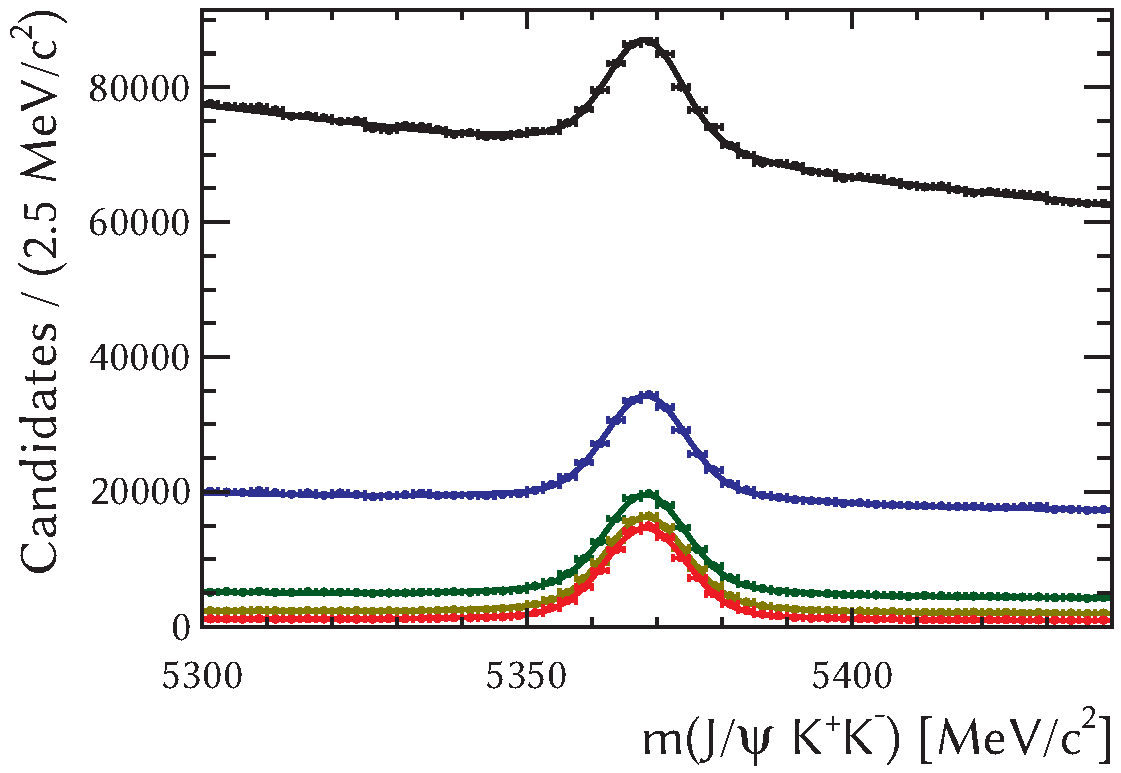
\includegraphics[width=0.7\textwidth]{graphics/analysis/JpsiKKMassSel}
  \caption{Distribution of \BstoJpsiKK{} decays in $\JpsiKK$ mass for different selection criteria.
           The data are shown as points, while the lines represent a model that consists of the sum of two Gaussian shapes (signal)
           and an exponential shape (combinatorial background).
           Subsequent selection criteria are applied in addition to previous criteria:
           black: stripping selection; blue: minimum quality of $\Bs$ decay-vertex reconstruction;
           green: minimum $\KK$ transverse momentum; yellow: minimum decay time; red: full offline selection.
           Notice that only a part of the total mass range is shown.}
  \label{fig:JpsiKKMassSel}
\end{figure}

For \BstoJpsiKK{} signal candidates this distribution is a peak around the value of the $\Bs$ mass of approximately 5367\unitsp\MeV. The
width of this peak is determined by the experimental resolution on the $\JpsiKK$-mass measurement. The background is mainly combinatorial
and follows an exponential distribution, which decreases slowly across the considered mass range. Because of the obvious difference in
distributions of $\JpsiKK$ mass for the signal and the background, this variable can be used to statistically separate the two
contributions.

The distribution of black data points in Figure~\ref{fig:JpsiKKMassSel} is for candidates that pass the stripping selection without further
requirements. A peak of signal candidates is visible on top of a large background distribution. To determine the numbers of signal and
background candidates, the surface areas underneath the peak and the exponential distribution are determined with a fit. The signal peak is
modelled with the sum of a narrow ($\sigma$\textapprox6\unitsp\MeV) and wide ($\sigma$\textapprox16\unitsp\MeV) Gaussian shape and the
background with and exponential shape. The fit yields approximately 123 thousand signal candidates, which corresponds to a signal fraction
of approximately one per cent.

In the rest frame of the $\Bs$, the momentum of the $\KK$ pair is approximately 1.6\unitsp\GeVc{} for signal decays. Boosting into the
frame of the detector, approximately along the beam axis, this translates into a typical transverse momentum above 1\unitsp\GeVc. The sum
of the transverse momentum components of two kaons that accidentally form a suitable $\KK$ vertex in combinatorial background is often not
sufficient to make a transverse momentum of 1\unitsp\GeVc. As a result, requiring this value as a minimum in the offline selection removes
about 74\% of the background, but only 6\% of the signal, with respect to the stripping selection where already a minimum of
0.5\unitsp\GeVc{} was required. The $\JpsiKK$-mass distribution with the $\KK$ transverse momentum requirement is shown by the blue points
in Figure~\ref{fig:JpsiKKMassSel}.

To estimate the position of the $\Bs$ decay vertex and the kinematics of the particles in the decay as well as possible, these variables
are determined from a fit. The fit takes the position of the primary vertex, the muon and kaon tracks, and the corresponding experimental
uncertainties as inputs and minimizes a $\chi^2$ function for the position of the decay vertex and its perpendicular distance to the flight
path of the $\Bs$, which should be equal to zero. The value of the $\chi^2$ function in its minimum is a measure of the quality of the fit,
i.e. of how well the four reconstructed particles form a $\Bs$ decay vertex. The fit will, in general, be good for signal candidates, which
results in small values of the $\chi^2$ function.

Requiring a $\chi^2$ smaller than five times the number of degrees of freedom in the vertex fit removes about 75\% of the background that
remains after requiring a minimum $\KK$ transverse momentum of 1\unitsp\GeVc. Approximately 8\% of the remaining signal is lost. The
distribution of decay candidates after the $\KK$ transverse momentum and vertex fit quality requirements is shown by the green points in
Figure~\ref{fig:JpsiKKMassSel}.

A third requirement that removes a significant part of the background is a minimum on the reconstructed value of the decay time. For most
of the background candidates the four particles originate directly from the primary vertex, which corresponds to vanishing decay time
within experimental resolution. The stripping selection already requires a minimum decay time of 0.2\unitsp{}ps. Requiring a minimum of
0.3\unitsp{}ps in addition to the stripping selection and the $\KK$ transverse momentum and vertex fit $\chi^2$ requirements removes about
54\% of the remaining background and 6\% of the signal. The distribution for remaining candidates is shown by the yellow points in
Figure~\ref{fig:JpsiKKMassSel}.

Finally applying the full offline selection removes another 62\% of the background and 6\% of the signal, leaving approximately 94
thousand signal candidates and 135 thousand background candidates for further analysis. This corresponds to a signal fraction of 41\% in
the full $\JpsiKK$-mass range of 5200--5550\unitsp\MeV{} after the full selection.

The final $\JpsiKK$-mass distribution is shown by the red points in Figure~\ref{fig:JpsiKKMassSel} and also in
Figure~\ref{fig:JpsiKKMass_DG}. The latter figure shows the distribution both in the 5300--5440\unitsp\MeV{} mass range on a linear
vertical scale (left) and in the full mass range on a logarithmic vertical scale. The signal and combinatorial background contributions as
determined in the fit are shown separately.

\begin{figure}[p]
  \centering
  \begin{subfigure}{0.65\textwidth}
    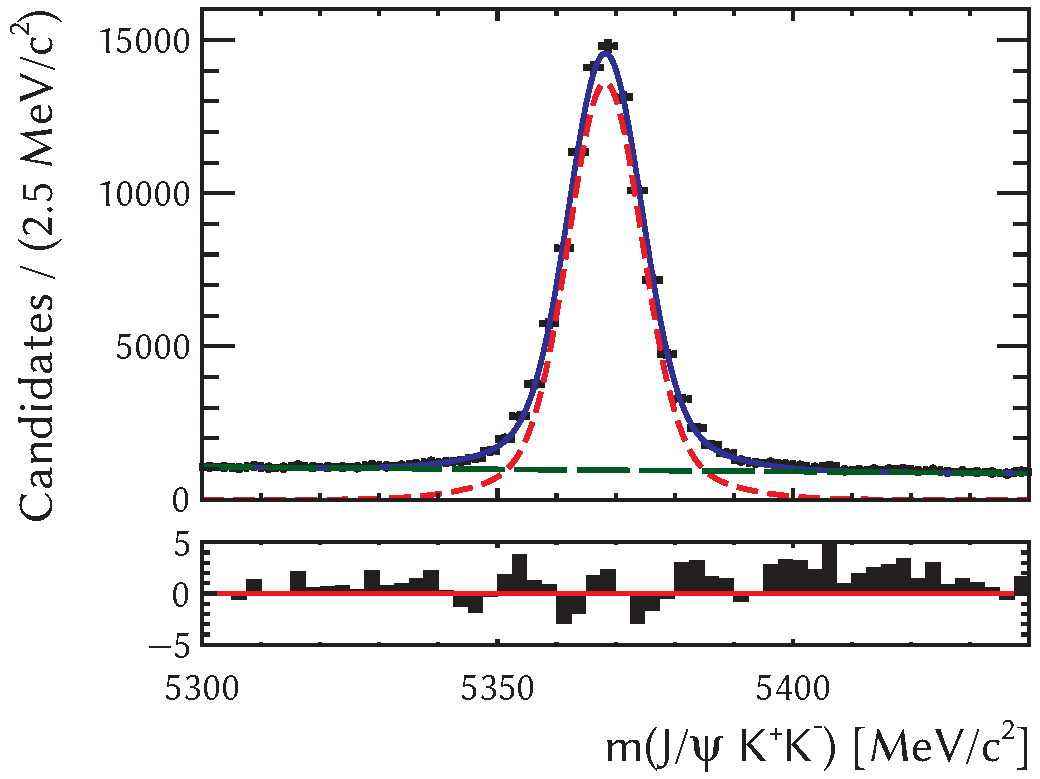
\includegraphics[width=\textwidth]{graphics/analysis/JpsiKKMass_DG_lin_resid}
    \caption{}
    \label{fig:JpsiKKMass_DG_lin}
  \end{subfigure}

  \vspace*{0.02\textwidth}
  \begin{subfigure}{0.65\textwidth}
    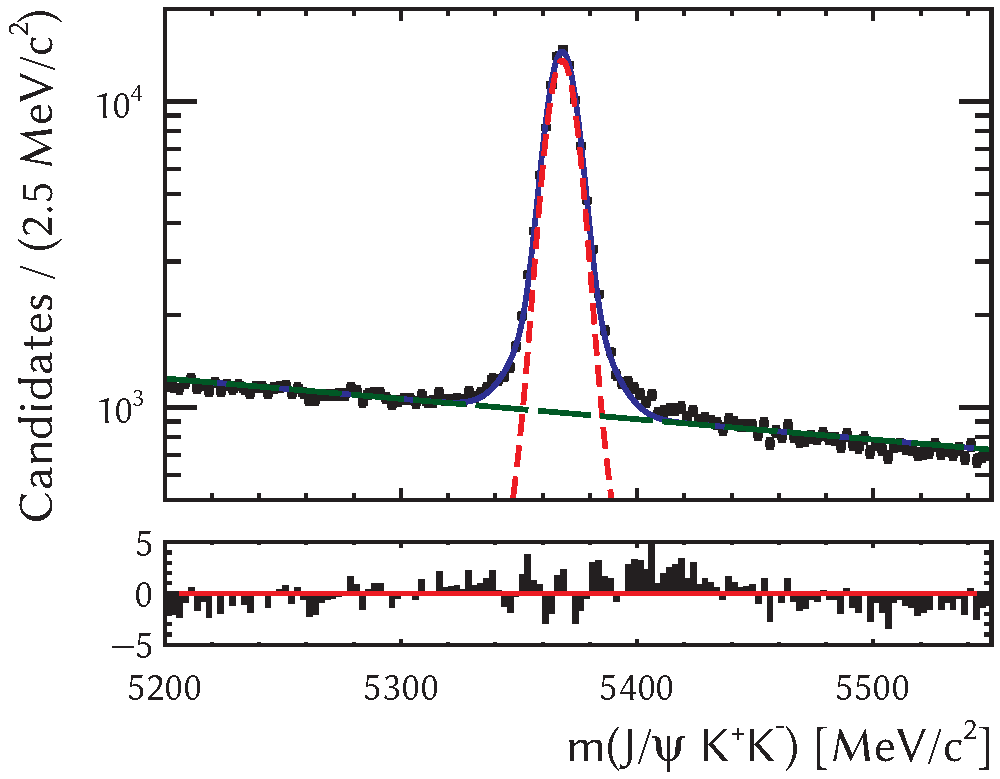
\includegraphics[width=\textwidth]{graphics/analysis/JpsiKKMass_DG_log_resid}
    \caption{}
    \label{fig:JpsiKKMass_DG_log}
  \end{subfigure}%
  \caption{Distribution of \BstoJpsiKK{} decay candidates in $\JpsiKK$ mass in
           (a) the signal mass range and
           (b) the full mass range on a logarithmic vertical scale.
           The black points show the distribution of the data and the blue, solid line shows a model that was fitted to the data.
           The model is the sum of two Gaussian shapes for the signal (shown by the red, short-dashed line)
           and an exponential shape for combinatorial background (shown by the green, long-dashed line).
           The panels below the distributions show the pulls of the data with respect to the model (see also text).}
  \label{fig:JpsiKKMass_DG}
\end{figure}

In the areas below the $\JpsiKK$-mass distributions in Figure~\ref{fig:JpsiKKMass_DG} the \emph{pull} is shown for each mass interval. The
pull is defined as the difference between the numbers of decay candidates that are observed (data) and expected (PDF), divided by the
estimated statistical uncertainty of the observed value. If the PDF describes the data correctly, this quantity is expected to be
distributed according to the standard normal distribution in the limit of a large number of decay candidates. Therefore, the pull
quantifies how well the model describes the data in each interval.

The pulls in Figure~\ref{fig:JpsiKKMass_DG_log} seem to indicate a problem with the mass model, since the PDF generally underestimates the
number of decay candidates in the region of the signal peak, while it overestimates the number of candidates towards the edges of the mass
range at 5200\unitsp\MeV{} and 5550\unitsp\MeV. This issue is mainly caused by misidentified backgrounds and will be addressed in
Section~\ref{subsec:ana_bkgSub_bkgSub}.

Notice from Figures~\ref{fig:JpsiKKMassSel} and \ref{fig:JpsiKKMass_DG} that the signal candidates are concentrated in a mass window of
approximately 60\unitsp\MeV, centred at the $\Bs$ mass, where the signal fraction is approximately 80\%. The regions to the left and the
right of this \emph{signal window} are called mass \emph{side bands} and contain mainly background candidates. The candidates in the side
bands are used to estimate the time and angular distribution of the combinatorial background and to subtract this from the total
distribution in the signal window to obtain the signal distribution. This procedure is described in the following section.


%%%%%%%%%%%%%%%%%%%%%%%%%%%%%%%%%%%
\subsection{Background Subtraction}
\label{subsec:ana_bkgSub_bkgSub}
%%%%%%%%%%%%%%%%%%%%%%%%%%%%%%%%%%%

The distribution of background decay candidates that remain after selection is subtracted from the total distribution by including
background candidates with negative weights in the data sample. For combinatorial background the most straightforward method of doing this
would be to give candidates in the signal region a weight equal to plus one and candidates in the $\JpsiKK$-mass side bands a small
negative weight, such that the contributions of background in the signal and side-band regions exactly cancel. Note that this assumes that
the background distribution in all variables of interest does not depend on the $\JpsiKK$ mass.

Because the definitions of the signal and side-band regions are rather arbitrary, a more sophisticated technique is applied. Although the
bulk of the signal decay candidates have a reconstructed $\JpsiKK$ mass in a region of approximately 60\unitsp\MeV{} around the $\Bs$ mass,
the tails of the signal mass distribution stretch beyond this mass window. Moreover, at the edges of the signal window the contribution of
background is larger than in the centre. To take these features of the mass distribution into account and estimate the contribution of
combinatorial background in the most optimal way, the candidate weights are not binary, but take a different value as a function of the
$\JpsiKK$ mass.

The weights for subtracting combinatorial background are computed with the \splot/\sfit{} technique~\cite{Pivk:2004ty,*Xie:2009rka}, which
takes the $\JpsiKK$-mass distributions of the signal and the background as inputs. The resulting candidate weights are called
\emph{\sweight[s]}, which are larger than one in the centre of the signal peak and gradually become smaller away from the peak and finally
become negative in the side bands.

The \splot/\sfit{} method assumes that, in addition to the background distribution, also the signal distribution in the variables of
interest does not depend on the $\JpsiKK$ mass. In other words, there can be no correlations between the $\JpsiKK$ mass and any other
variable that is to be analysed for the signal and background distributions separately. Note that, in general, there are correlations for
the sum of signal and background.

Before fitting the distribution of signal and combinatorial-background candidates and computing \sweight[s], contributions from other
backgrounds are subtracted by adding decay candidates with negative weights to the data sample. Two additional backgrounds are considered,
both originating from the misidentification of particles in the detector: \BdtoJpsiKstKpi{} and \LbtoJpsipK. Because the detected particles
for these processes originate from decays of unstable particles (resonances), these contributions are also called \emph{resonant
backgrounds}.

\begin{figure}[tb]
  \centering
  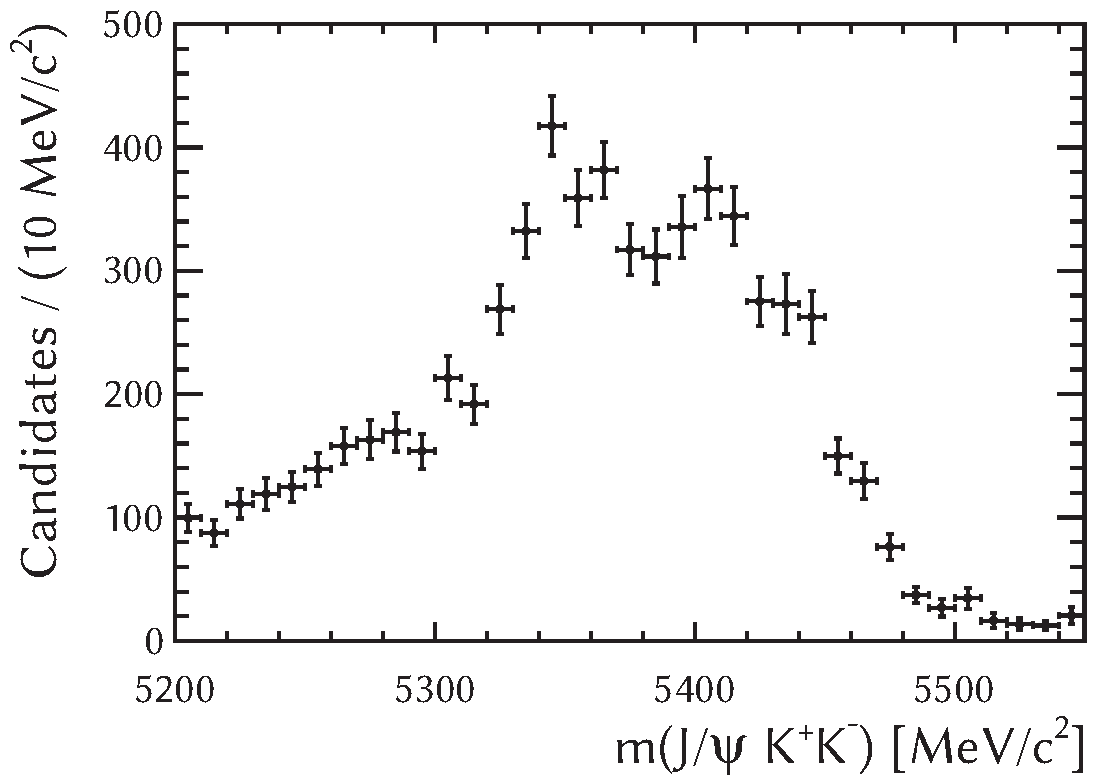
\includegraphics[width=0.5\textwidth]{graphics/analysis/JpsiKKMass_peakBkg}
  \caption{Distribution of weighted simulated resonant-background \BstoJpsiKK{} decay candidates in $\JpsiKK$ mass in the full mass range.}
  \label{fig:JpsiKKMass_peakBkg}
\end{figure}

\begin{figure}[p]
  \centering
  \begin{subfigure}{0.65\textwidth}
    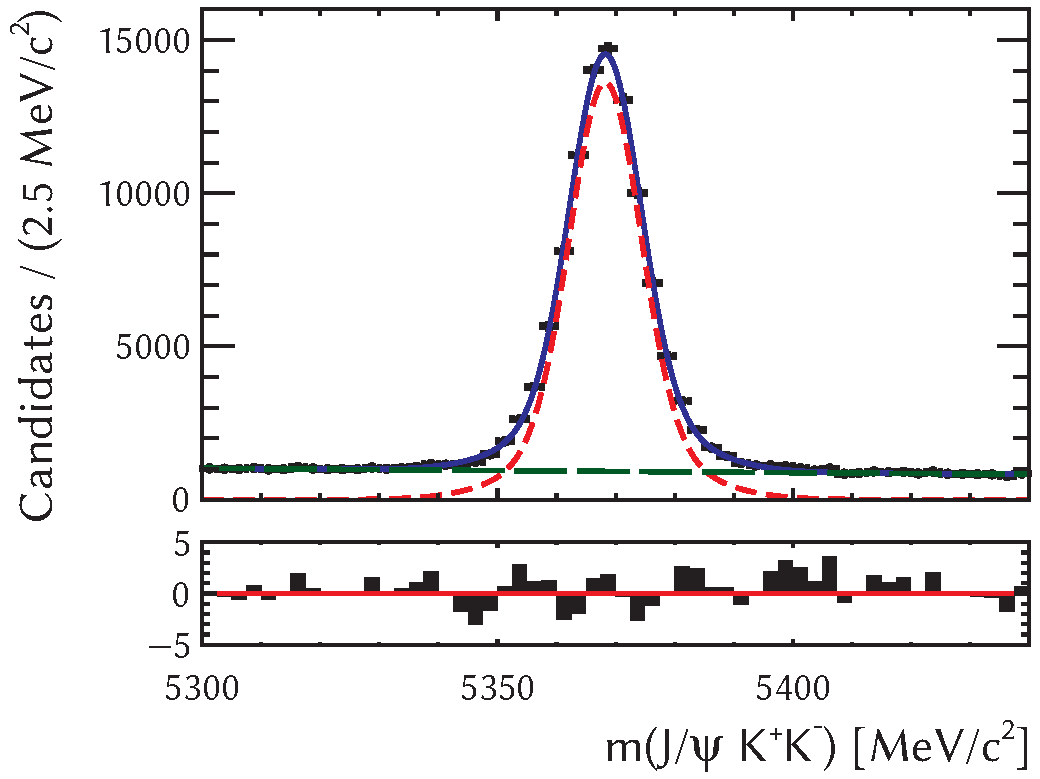
\includegraphics[width=\textwidth]{graphics/analysis/JpsiKKMass_DG_bkgSub_lin_resid}
    \caption{}
    \label{fig:JpsiKKMass_I2_lin}
  \end{subfigure}

  \vspace*{0.02\textwidth}
  \begin{subfigure}{0.65\textwidth}
    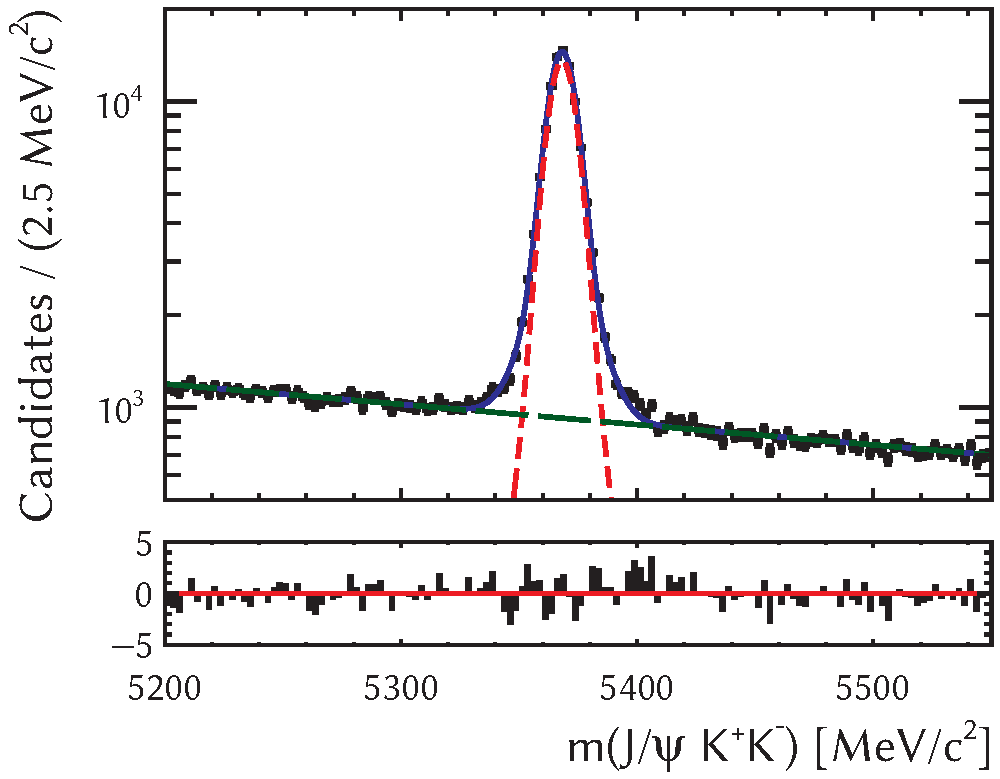
\includegraphics[width=\textwidth]{graphics/analysis/JpsiKKMass_DG_bkgSub_log_resid}
    \caption{}
    \label{fig:JpsiKKMass_I2_log}
  \end{subfigure}%
  \caption{Distribution of \BstoJpsiKK{} decay candidates in $\JpsiKK$ mass after subtracting resonant backgrounds in
           (a) the signal mass range and
           (b) the full mass range on a logarithmic vertical scale.
           The black points show the distribution of the data and the blue, solid line shows a model that was fitted to the data.
           The model is the sum of two Gaussian shapes for the signal (shown by the red, short-dashed line)
           and an exponential shape for combinatorial background (shown by the green, long-dashed line).
           The panels below the distributions show the pulls of the data with respect to the model.}
  \label{fig:JpsiKKMass_DG_bkgSub}
\end{figure}

Figure~\ref{fig:JpsiKKMass_peakBkg} shows the sum of the reconstructed $\JpsiKK$-mass distributions for the two resonant backgrounds. They
form a broad structure, without features that clearly distinguish these backgrounds from the signal and from combinatorial background.
Therefore, the resonant backgrounds are subtracted by adding simulated \BdtoJpsiKstKpi{} and \LbtoJpsipK{} decay candidates to the data
sample with negative weights that represent the estimated amount of real resonant-background data, in total approximately seven thousand
candidates.  Uncertainties in the numbers of background candidates and their distributions lead to systematic uncertainties in the final
parameter estimates, as will be discussed in Section~\ref{sec:result_syst}.

The $\JpsiKK$-mass distribution after subtracting the two resonant backgrounds is shown in Figure~\ref{fig:JpsiKKMass_DG_bkgSub}. Comparing
to Figure~\ref{fig:JpsiKKMass_DG}, it can be seen from the pulls that the PDF follows the data more closely. The systematic
underestimates of the numbers of decay candidates in the signal region and the overestimates in the side-band regions have been reduced. It
appears, however, that this effect is still partially present. Moreover, the pulls in the signal region seem to be large than one would
expect.

\begin{figure}[tbp]
  \centering
  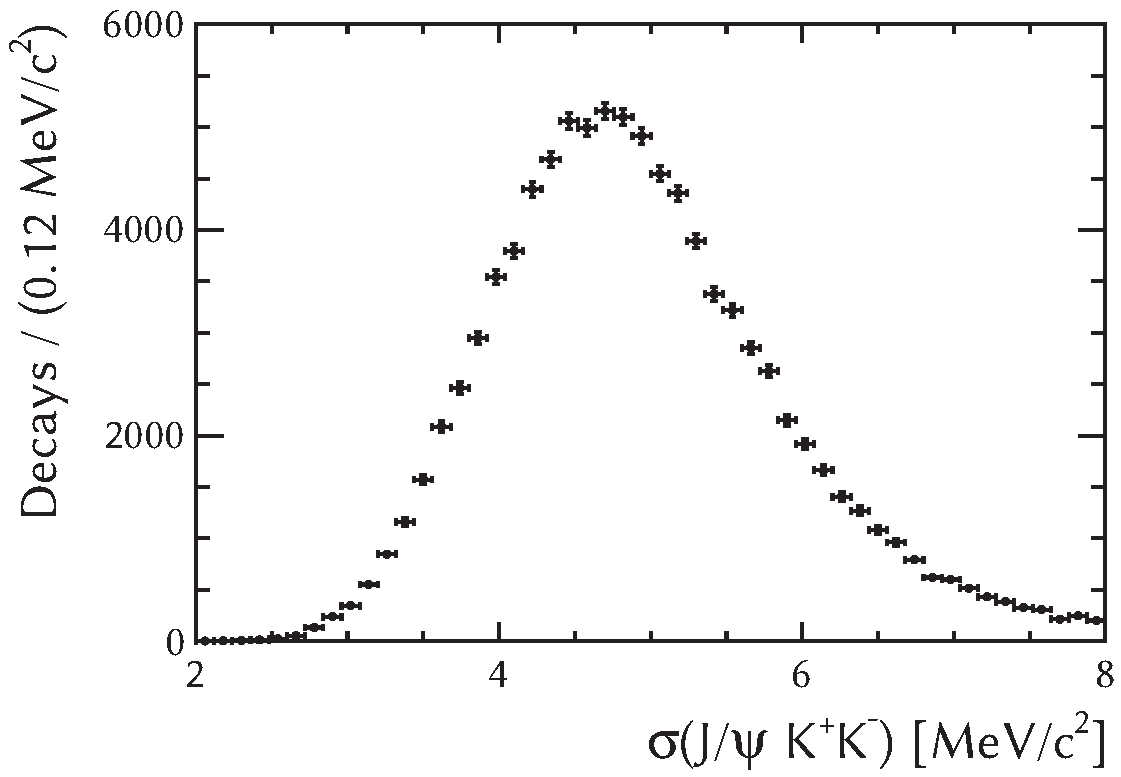
\includegraphics[width=0.5\textwidth]{graphics/analysis/JpsiKKMassErr}
  \caption{Distribution of \BstoJpsiKK{} signal decays in the estimated $\JpsiKK$-mass uncertainty.}
  \label{fig:JpsiKKMassErr}
\end{figure}

To address these issues, the double-Gaussian signal model is replaced by a more sophisticated model for the mass resolution.
Figure~\ref{fig:JpsiKKMassErr} shows the distribution of the estimated uncertainty in the $\JpsiKK$-mass measurement for each decay. This
distribution does not feature a structure with two sharp peaks, as would be expected for a double-Gaussian mass model, but is instead described
by one broad peak. To describe the resulting mass distribution a double-sided Hypatia function with a symmetric core~\cite{Santos:2013gra} is
used, which is designed to describe the effects of an experimental resolution that varies from decay candidate to decay candidate.

The Hypatia function is defined by
\begin{subequations}
\begin{equation}
  I(m) \equiv
  \begin{cases}
    \left[(m-\mu)^{2} + \delta^{2}\right]^{\frac{1}{2} \lambda - \frac{1}{4}}
          \!\!\!\!& K_{\lambda - \frac{1}{2}}\big(\alpha \sqrt{(m-\mu)^2 + \delta^2}\big) \\
          &\text{if}\ \ -a_L\,\sigma < m - \mu < +a_R\,\sigma \\
    \frac{A_L}{(B_L - m+\mu)^{n_L}} &\text{if}\ \ m - \mu < -a_L\,\sigma \\
    \frac{A_R}{(B_R + m-\mu)^{n_R}} &\text{if}\ \ m - \mu > +a_R\,\sigma
  \end{cases}
\end{equation}
with
\begin{equation}
  \alpha\equiv\frac{1}{\sigma}\sqrt{\frac{\zeta\, K_{\lambda+1}(\zeta)}{K_\lambda(\zeta)}}
  \qquad\text{and}\qquad
  \delta\equiv\sigma\sqrt{\frac{\zeta\,K_\lambda(\zeta)}{K_{\lambda+1}(\zeta)}} \ ,
\end{equation}
\end{subequations}
where $m$ is the mass variable and $K_{\nu}(z)$ the modified Bessel function of the second kind. The parameter $\mu$ controls the position
of the mass peak, $\sigma$ controls the width of its core, and $\lambda$ and $\zeta$ control the shape of its core. The double-sided
Hypatia function has an enhanced tail on both the left and the right side of the mass peak, the positions and shapes of which are
controlled by the parameters $a_{L/R}$ and $n_{L/R}$, respectively. The parameters $A_{L/R}$ and $B_{L/R}$ are obtained by imposing
continuity and differentiability at the points of transition between the core of the function and its tails.

The Hypatia parameters $\lambda$\textapprox\tm2.5, 0\textlt$\zeta$\textlt0.5, $a_{L/R}$\textapprox2.5, and 0\textlt$n_{L/R}$\textlt3 are
determined from simulated \BstoJpsiphi{} signal decays. Only the mean ($\mu$\textapprox5368\unitsp\MeV) and the width
($\sigma$\textapprox8\unitsp\MeV) of the core are determined in a fit to the real data. Consequently, the number of free parameters in the
Hypatia model is smaller than in the double-Gaussian model, for which the mean, the two widths, and the relative contribution of the two
functions were free parameters.

The result of a fit with the Hypatia signal model and an exponential shape for the combinatorial background is shown in
Figure~\ref{fig:JpsiKKMass_I2_bkgSub}. The improvement with the Hypatia model can be seen from the pulls, which are smaller in the signal
region and more symmetrically distributed around zero in comparison to Figure~\ref{fig:JpsiKKMass_DG_bkgSub}.

\begin{figure}[p]
  \centering
  \begin{subfigure}{0.65\textwidth}
    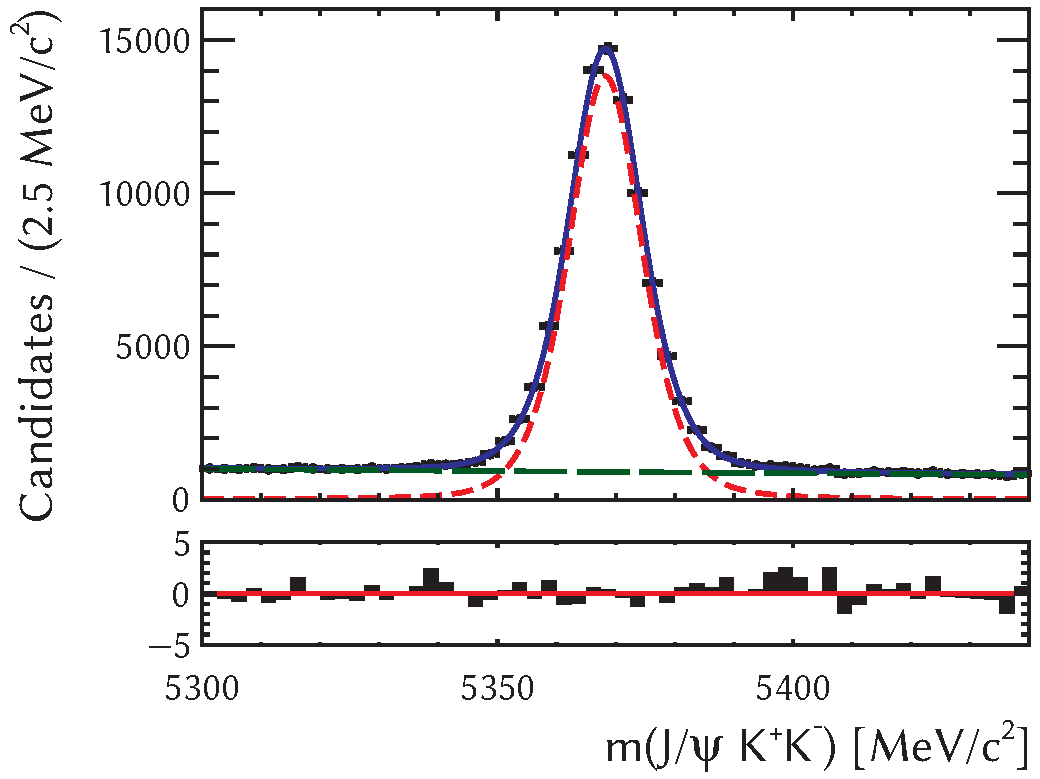
\includegraphics[width=\textwidth]{graphics/analysis/JpsiKKMass_I2_bkgSub_lin_resid}
    \caption{}
    \label{fig:JpsiKKMass_I2_bkgSub_lin}
  \end{subfigure}

  \vspace*{0.02\textwidth}
  \begin{subfigure}{0.65\textwidth}
    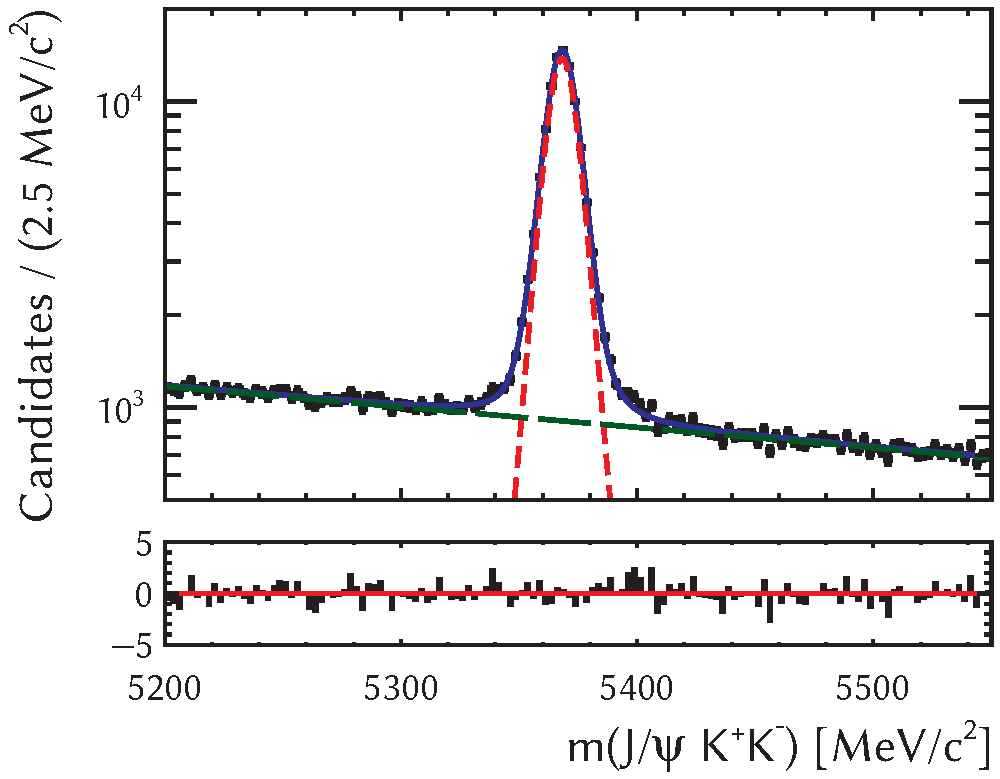
\includegraphics[width=\textwidth]{graphics/analysis/JpsiKKMass_I2_bkgSub_log_resid}
    \caption{}
    \label{fig:JpsiKKMass_I2_bkgSub_log}
  \end{subfigure}%
  \caption{Distribution of \BstoJpsiKK{} decay candidates in $\JpsiKK$ mass after subtracting resonant backgrounds in
           (a) the signal mass range and
           (b) the full mass range on a logarithmic vertical scale.
           The black points show the distribution of the data and the blue, solid line shows a model that was fitted to the data.
           The model is the sum of an Hypatia shape for the signal (shown by the red, short-dashed line)
           and an exponential shape for combinatorial background (shown by the green, long-dashed line).
           The panels below the distributions show the pulls of the data with respect to the model.}
  \label{fig:JpsiKKMass_I2_bkgSub}
\end{figure}

Studies of the $\JpsiKK$-mass shape of signal decays have shown that it depends on the $\KK$ invariant mass. Therefore, the parameters of
the mass model are determined separately in the $\KK$-mass intervals that are also used in the final time and angular model to determine
the trend in the difference between the $\Jpsiphi$ and $\KK$ S-wave phases (see Section~\ref{subsec:pheno_equations_symmetry}).
Combinatorial background is subtracted separately for each interval.

The $\KK$-mass intervals are defined in Table~\ref{tab:KKBins}. In addition to this binning, the table also lists the final numbers of
signal and combinatorial-background decays and the weighted-likelihood correction factors (see Section~\ref{subsec:ana_fit_weights}) for
each interval.

\begin{table}[p]
  \centering
  \caption{Definition of the intervals in $\KK$ invariant mass. For each interval, the numbers of signal and background candidates,
           and the correction factors for a likelihood with weighted candidates for the 2011 and 2012 runs
           (see Section~\ref{subsec:ana_fit_weights}) are shown.}
  \label{tab:KKBins}
  \begin{tabular}{cccccc}
    \hline
    int.  &  range [\MeV]          &  signal [\tenpow{3}]  &  comb. bkg. [\tenpow{3}]  &  $\alpha_{2011}$  &  $\alpha_{2012}$  \\
    \hline
    1    &  \phantom{0}990--1008  &  \phantom{0}2         &  23                          &  0.42          &  0.39             \\
    2    &  1008--1016            &  10                   &  15                          &  0.79          &  0.76             \\
    3    &  1016--1020            &  35                   &  11                          &  0.94          &  0.93             \\
    4    &  1020--1024            &  28                   &  12                          &  0.92          &  0.92             \\
    5    &  1024--1032            &  13                   &  19                          &  0.77          &  0.77             \\
    6    &  1032--1050            &  \phantom{0}8         &  46                          &  0.51          &  0.51             \\
    \hline
  \end{tabular}
\end{table}

\begin{table}[p]
  \centering
  \caption{Parameters of the $\JpsiKK$-mass model that is used for background subtraction.
           The subscripts on the parameters refer to the interval in $\KK$ mass (1--6),
           the HLT2-biased/not-HLT2-biased category (b and nb, respectively), and the run period (2011 and 2012).}
  \label{tab:JpsiKKMassPars}
  \begin{tabular}{ccc}
    \hline
    par.                      &  value            &  stat. uncert.  \\
                              &  [\MeV]           &  [\MeV]         \\
    \hline
    $\mu_1$                   &  5368.47          &  0.25           \\
    $\mu_2$                   &  5367.79          &  0.09           \\
    $\mu_3$                   &  5367.93          &  0.04           \\
    $\mu_4$                   &  5368.65          &  0.05           \\
    $\mu_5$                   &  5368.69          &  0.08           \\
    $\mu_6$                   &  5368.39          &  0.13           \\
    $\sigma_{1,\mathrm{b}}$   &  \phantom{0}8.9   &  0.4            \\
    $\sigma_{2,\mathrm{b}}$   &  \phantom{0}8.23  &  0.11           \\
    $\sigma_{3,\mathrm{b}}$   &  \phantom{0}7.98  &  0.05           \\
    $\sigma_{4,\mathrm{b}}$   &  \phantom{0}7.87  &  0.05           \\
    $\sigma_{5,\mathrm{b}}$   &  \phantom{0}8.40  &  0.10           \\
    $\sigma_{6,\mathrm{b}}$   &  \phantom{0}8.90  &  0.18           \\
    $\sigma_{1,\mathrm{nb}}$  &  14.7             &  3.4            \\
    $\sigma_{2,\mathrm{nb}}$  &  \phantom{0}6.2   &  0.9            \\
    $\sigma_{3,\mathrm{nb}}$  &  \phantom{0}7.0   &  0.4            \\
    $\sigma_{4,\mathrm{nb}}$  &  \phantom{0}7.0   &  0.5            \\
    $\sigma_{5,\mathrm{nb}}$  &  \phantom{0}7.1   &  0.9            \\
    $\sigma_{6,\mathrm{nb}}$  &  \phantom{0}7.6   &  1.8            \\
    \hline
  \end{tabular}%
  \hspace*{15pt}%
  \begin{tabular}{ccc}
    \hline
    par.                         &  value            &  stat. uncert.  \\
     &  [$c$\textsuperscript{2}/MeV]  &  [$c$\textsuperscript{2}/MeV]  \\
    \hline
    $\gamma_{\mathrm{b},2011}$   &  0.00176  &  0.00006  \\
    $\gamma_{\mathrm{b},2012}$   &  0.00153  &  0.00003  \\
    $\gamma_{\mathrm{nb},2011}$  &  0.00032  &  0.00024  \\
    $\gamma_{\mathrm{nb},2012}$  &  0.00054  &  0.00015  \\
    \hline
    & & \\ & & \\ & & \\ & & \\ & & \\ & & \\ & & \\ & & \\ & & \\ & & \\ & & \\ & & \\ & & \\ & & \\
  \end{tabular}
\end{table}

There is no evidence for the $\JpsiKK$-mass distribution of the background to depend on the $\KK$ mass, but it does depend on two other
variables in the data. The background distribution is found to be different for the 2011 and 2012 run periods and for decay candidates that
are selected by the biased HLT2 trigger and candidates that are exclusively selected by the unbiased HLT2 trigger. Because these two
variables are used in the measurement and implementation of the decay-time efficiency function (see Section~\ref{subsec:ana_time_acc}),
background subtraction is also performed separately in the four categories associated to these variables. In addition, the  width of the
signal peak is determined separately for HLT2-biased and not-HLT2-biased candidates.

The final parameters of the $\JpsiKK$-mass model that were determined from the real data are listed in Table~\ref{tab:JpsiKKMassPars},
where the exponential function for the background mass distribution is described by $e^{-\gamma m}$, where $\gamma$ is a free parameter
that is different for the 2011 and 2012 runs and for HLT2-biased and not-HLT2-biased candidates. The number of signal decays determined
with this model is 96 thousand and the number of combinatorial-background decays 127 thousand.

To check whether the decay time and decay angles are correlated with the $\JpsiKK$ mass, the mass distribution is plotted for different
intervals in time and angles. A correlation appears when considering $\cthetal$, for which the distribution is shown in the
intervals $|\cthetal|$\textlt0.25, 0.25\textle$|\cthetal|$\textlt0.7, and $|\cthetal|$\textge0.7 in
Figure~\ref{fig:JpsiKKMass_I2_bkgSub_ctl}. In all three cases the nominal mass model from Figure~\ref{fig:JpsiKKMass_I2_bkgSub} is shown.
\begin{figure}[tbp]
  \centering
  \begin{subfigure}{0.49\textwidth}
    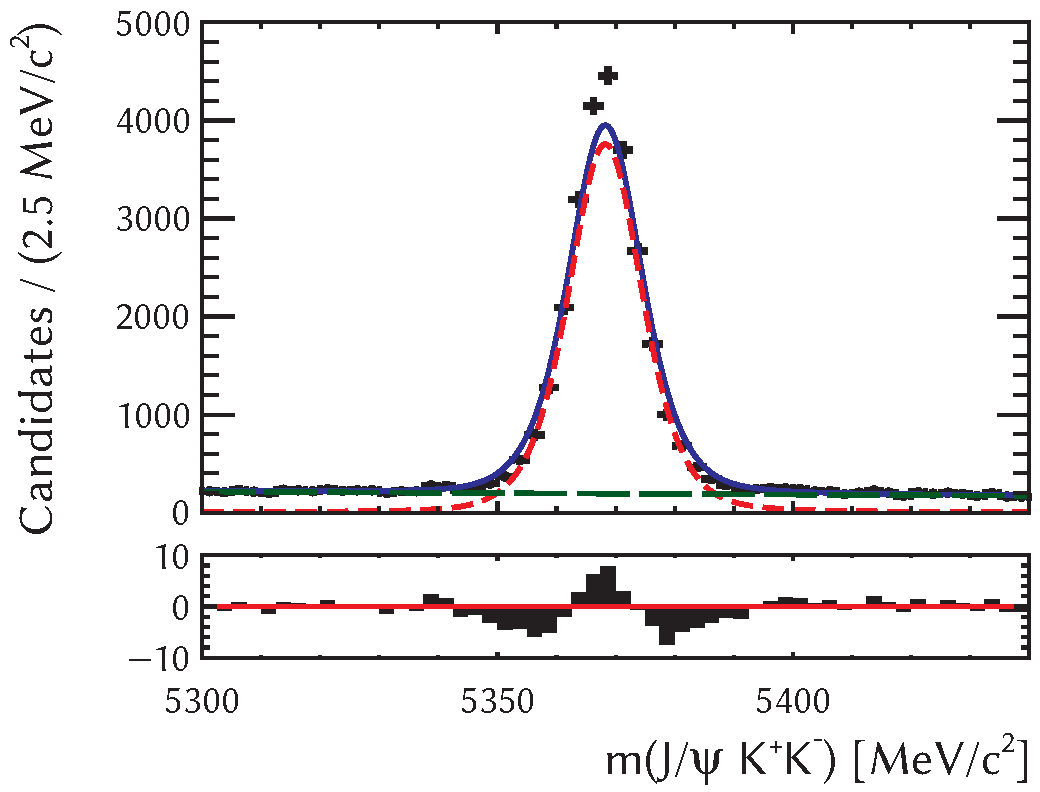
\includegraphics[width=\textwidth]{graphics/analysis/JpsiKKMass_I2_bkgSub_ctl2_lin_resid}
    \caption{}
    \label{fig:JpsiKKMass_I2_bkgSub_ctl2_lin}
  \end{subfigure}%
  \hfill%
  \begin{subfigure}{0.49\textwidth}
    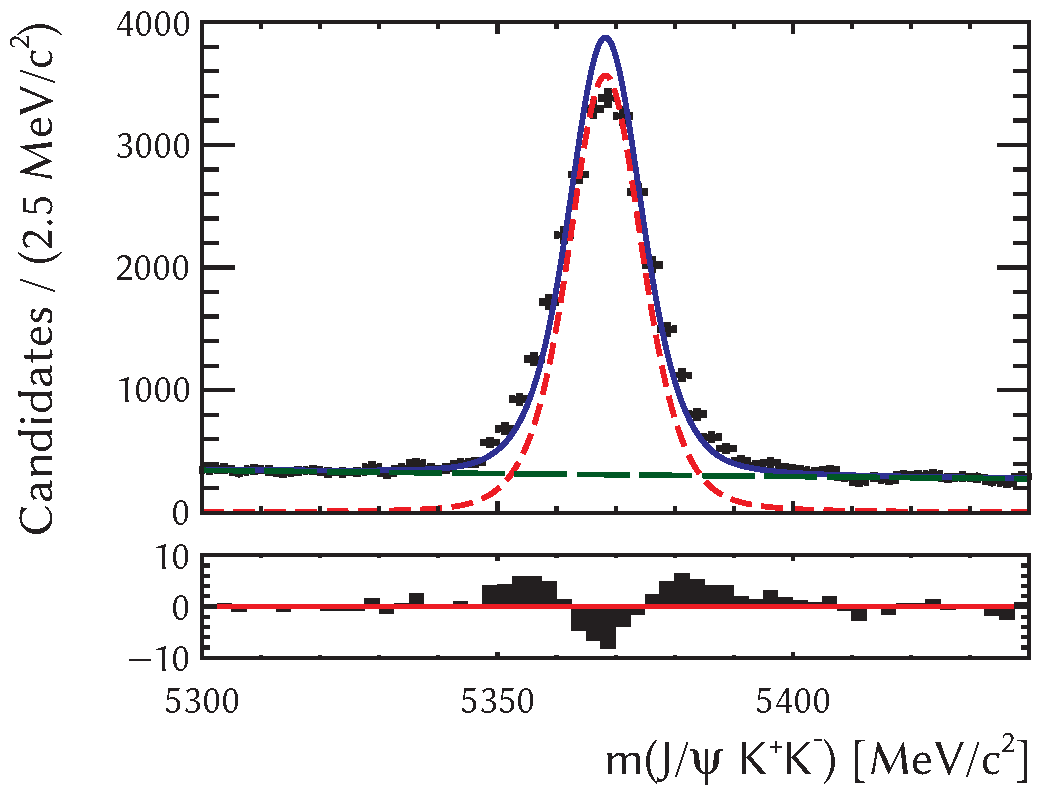
\includegraphics[width=\textwidth]{graphics/analysis/JpsiKKMass_I2_bkgSub_ctl04_lin_resid}
    \caption{}
    \label{fig:JpsiKKMass_I2_bkgSub_ctl04_lin}
  \end{subfigure}

  \vspace*{0.02\textwidth}
  \begin{subfigure}{0.49\textwidth}
    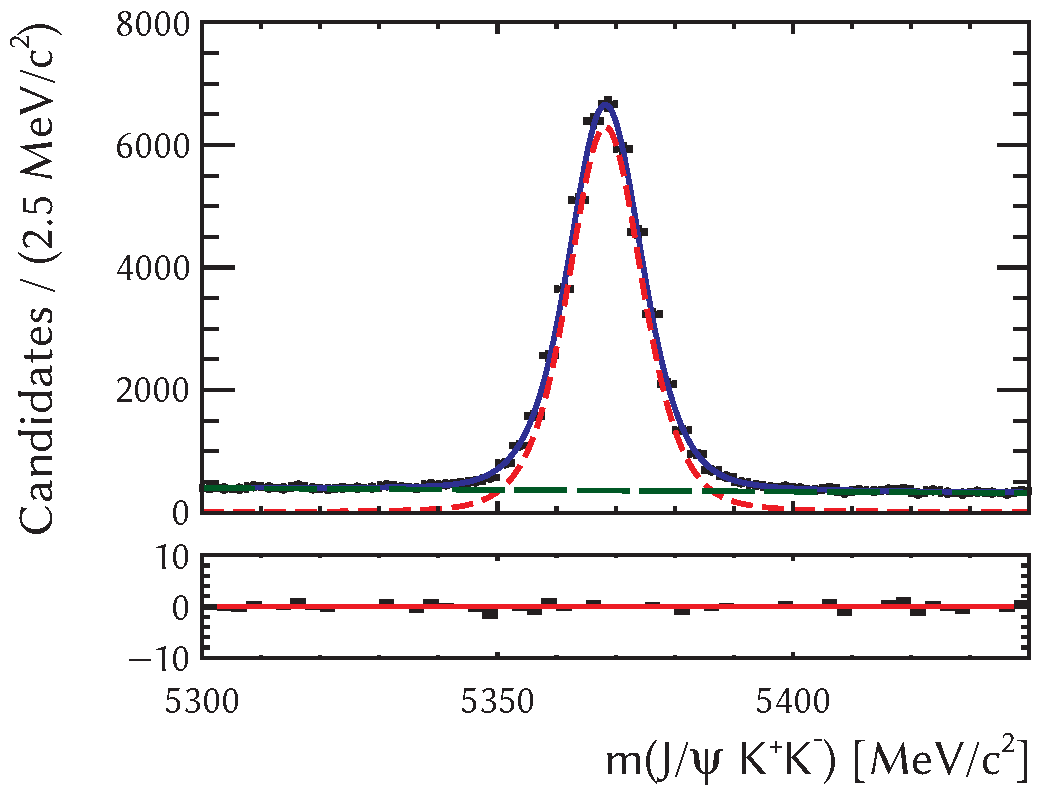
\includegraphics[width=\textwidth]{graphics/analysis/JpsiKKMass_I2_bkgSub_ctl13_lin_resid}
    \caption{}
    \label{fig:JpsiKKMass_I2_bkgSub_ctl13}
  \end{subfigure}%
  \caption{Distribution of \BstoJpsiKK{} decay candidates in $\JpsiKK$ mass after subtracting resonant backgrounds
           in intervals of $\cthetal$, where the shape of the model is set to the nominal shape
           from Figure~\ref{fig:JpsiKKMass_I2_bkgSub}.
           (a) $|\cthetal|$\textlt0.25,
           (b) $|\cthetal|$\textge0.7,
           (c) 0.25\textle$|\cthetal|$\textlt0.7.
           (Compare to the nominal mass distribution in Figure~\ref{fig:JpsiKKMass_I2_bkgSub})}
  \label{fig:JpsiKKMass_I2_bkgSub_ctl}
\end{figure}

\begin{figure}[tbp]
  \centering
  \begin{subfigure}{0.49\textwidth}
    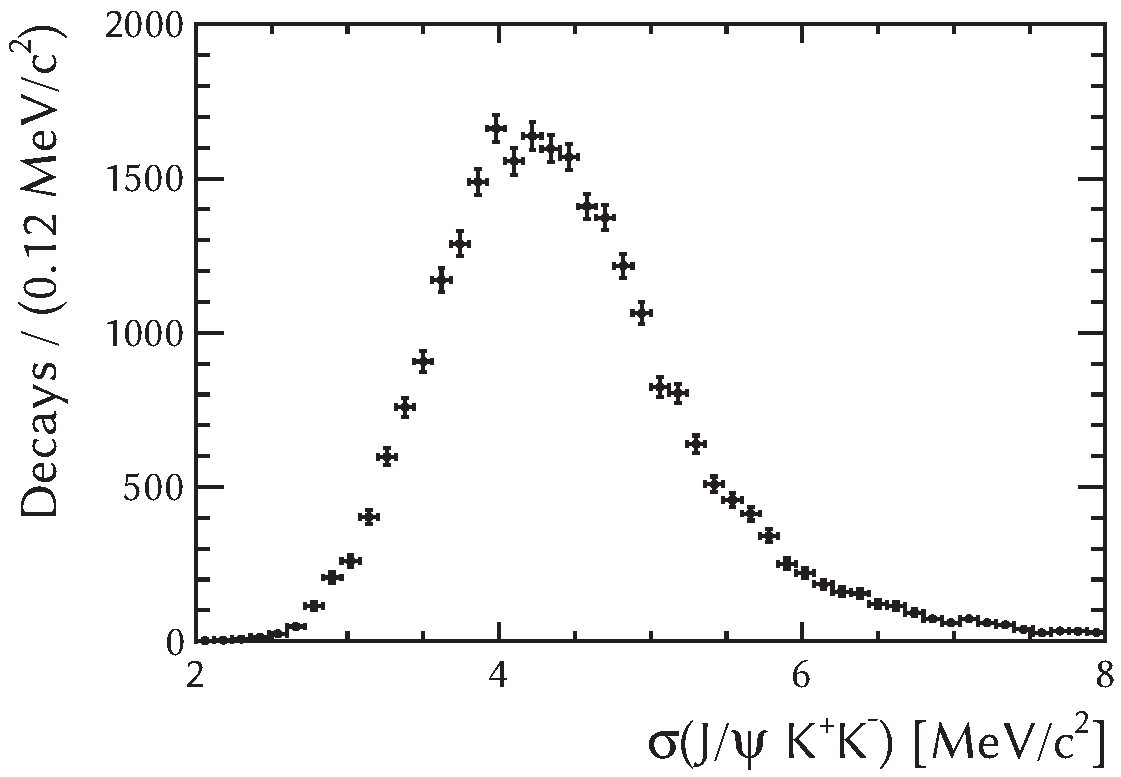
\includegraphics[width=\textwidth]{graphics/analysis/JpsiKKMassErr_left}
    \caption{}
    \label{fig:JpsiKKMassErr_left}
  \end{subfigure}%
  \hfill%
  \begin{subfigure}{0.49\textwidth}
    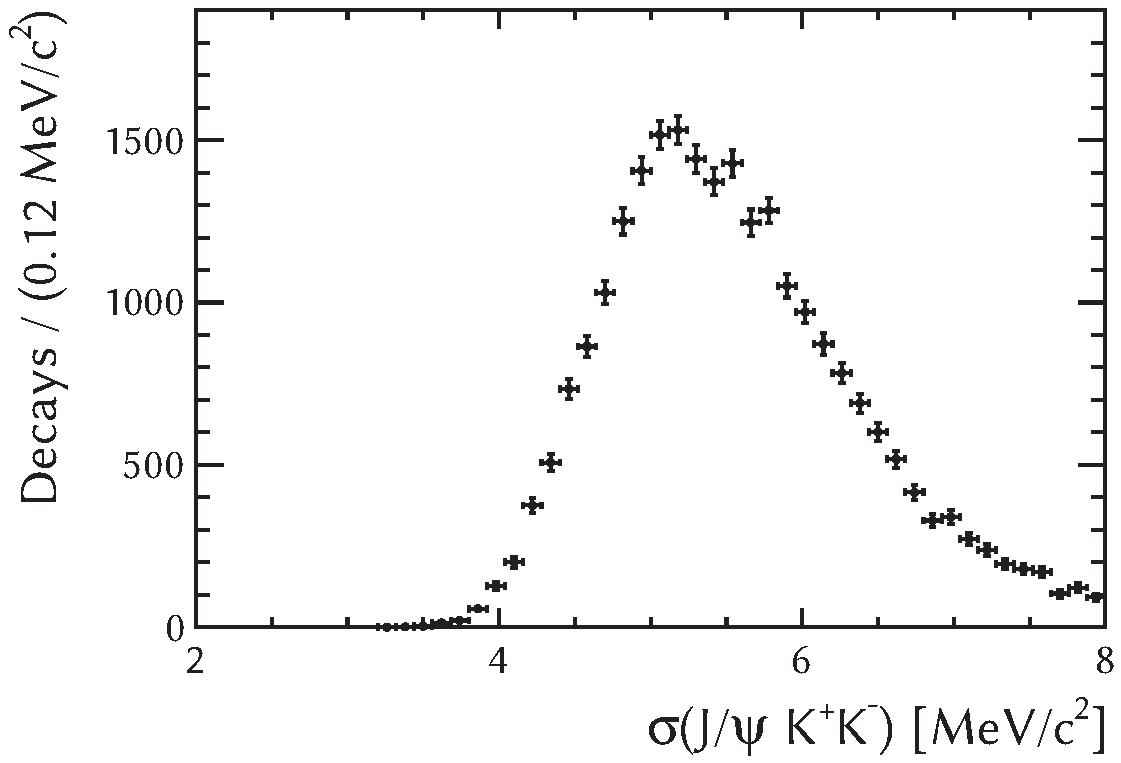
\includegraphics[width=\textwidth]{graphics/analysis/JpsiKKMassErr_right}
    \caption{}
    \label{fig:JpsiKKMassErr_right}
  \end{subfigure}

  \vspace*{0.02\textwidth}
  \begin{subfigure}{0.49\textwidth}
    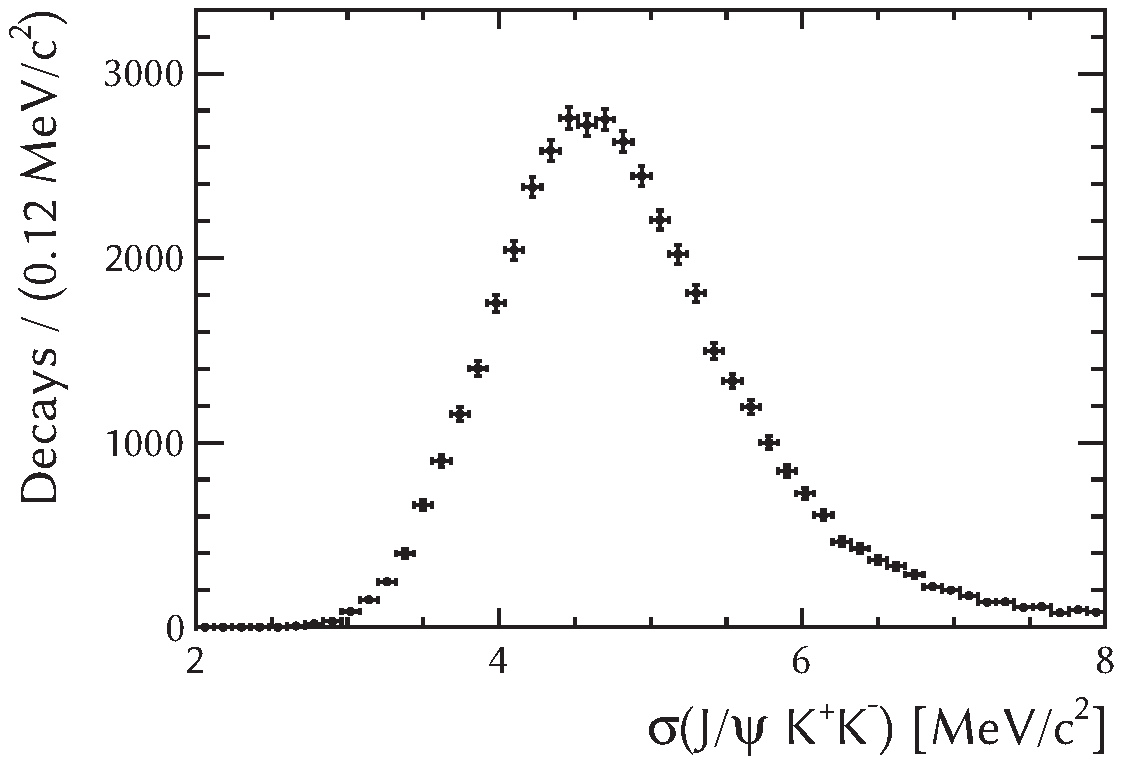
\includegraphics[width=\textwidth]{graphics/analysis/JpsiKKMassErr_middle}
    \caption{}
    \label{fig:JpsiKKMassErr_middle}
  \end{subfigure}%
  \caption{Distribution of \BstoJpsiKK{} signal decays in the estimated $\JpsiKK$-mass uncertainty in different intervals of $\cthetal$:
           (a) $|\cthetal|$\textlt0.25,
           (b) $|\cthetal|$\textge0.7, and
           (c) 0.25\textle$|\cthetal|$\textlt0.7.}
  \label{fig:JpsiKKMassErr_ctlBins}
\end{figure}

\begin{figure}[p]
  \centering
  \begin{subfigure}{0.49\textwidth}
    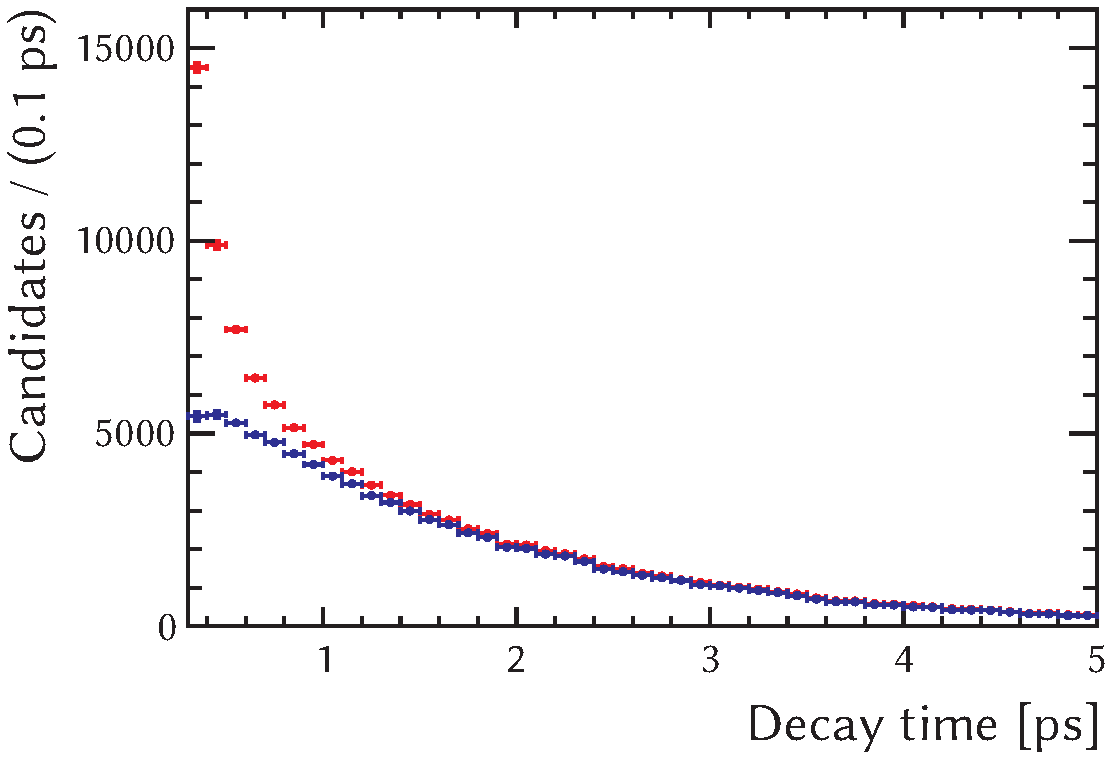
\includegraphics[width=\textwidth]{graphics/analysis/time_bkgSub}
    \caption{}
    \label{fig:timeBkgSub}
  \end{subfigure}%
  \hfill%
  \begin{subfigure}{0.49\textwidth}
    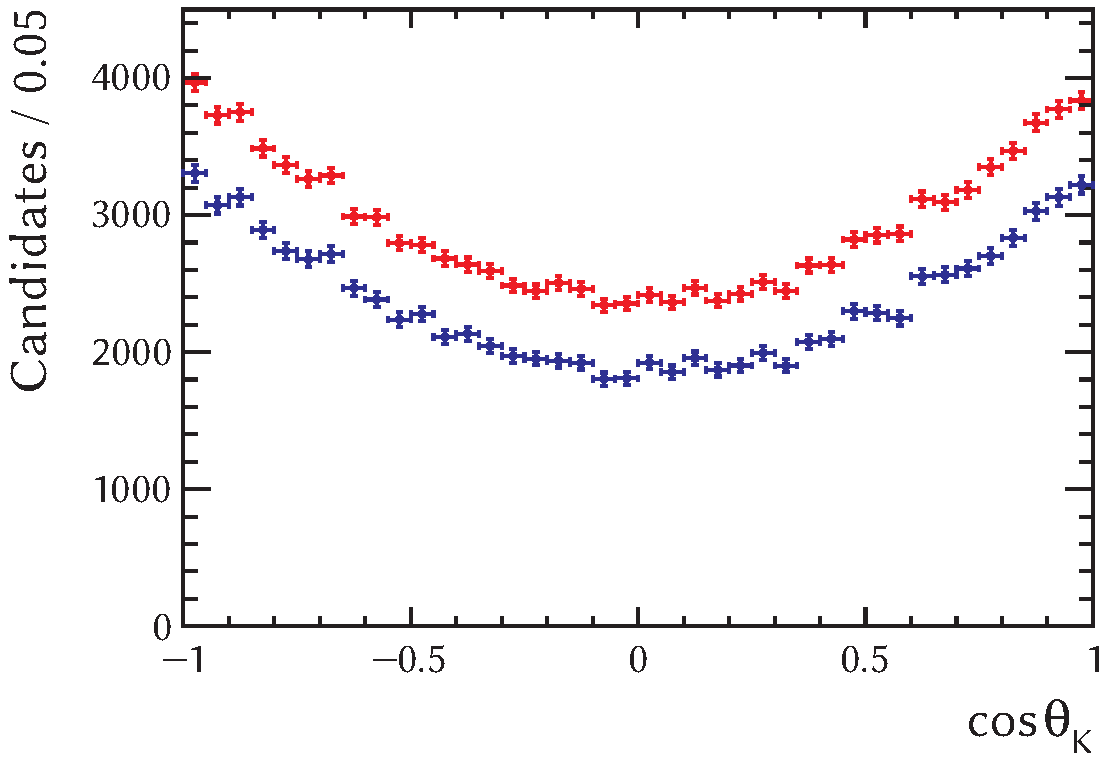
\includegraphics[width=\textwidth]{graphics/analysis/ctk_bkgSub}
    \caption{}
    \label{fig:ctkBkgSub}
  \end{subfigure}

  \vspace*{0.02\textwidth}
  \begin{subfigure}{0.49\textwidth}
    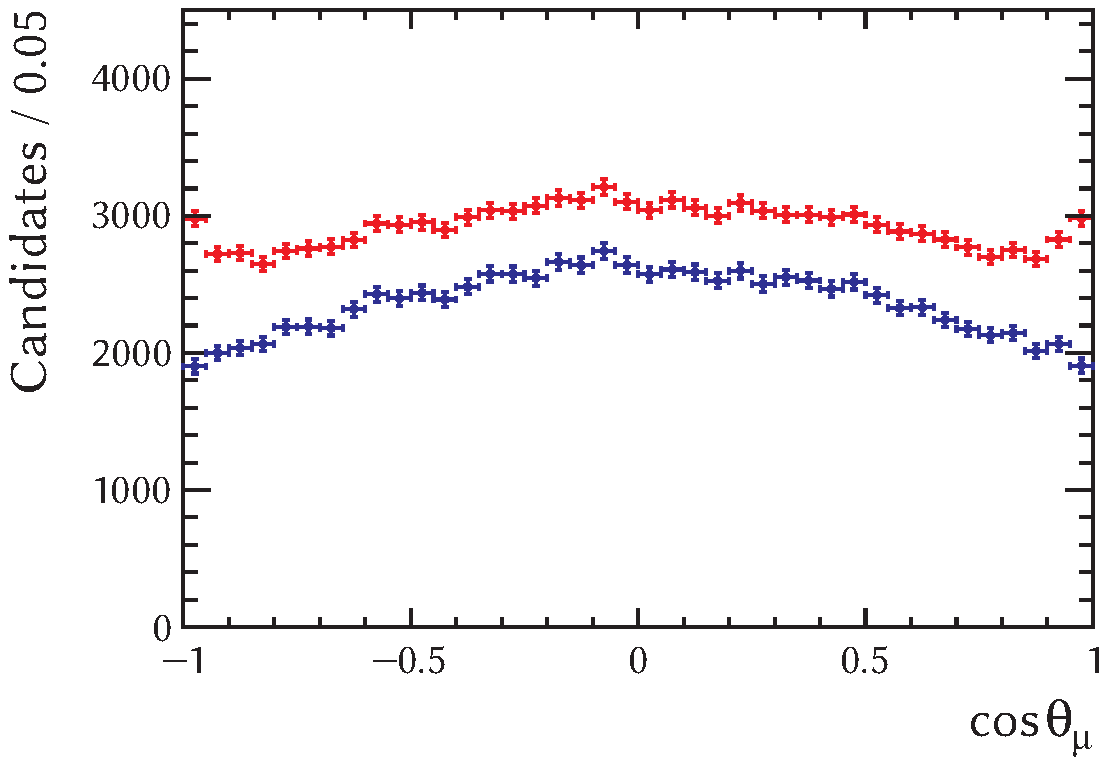
\includegraphics[width=\textwidth]{graphics/analysis/ctl_bkgSub}
    \caption{}
    \label{fig:ctlBkgSub}
  \end{subfigure}%
  \hfill%
  \begin{subfigure}{0.49\textwidth}
    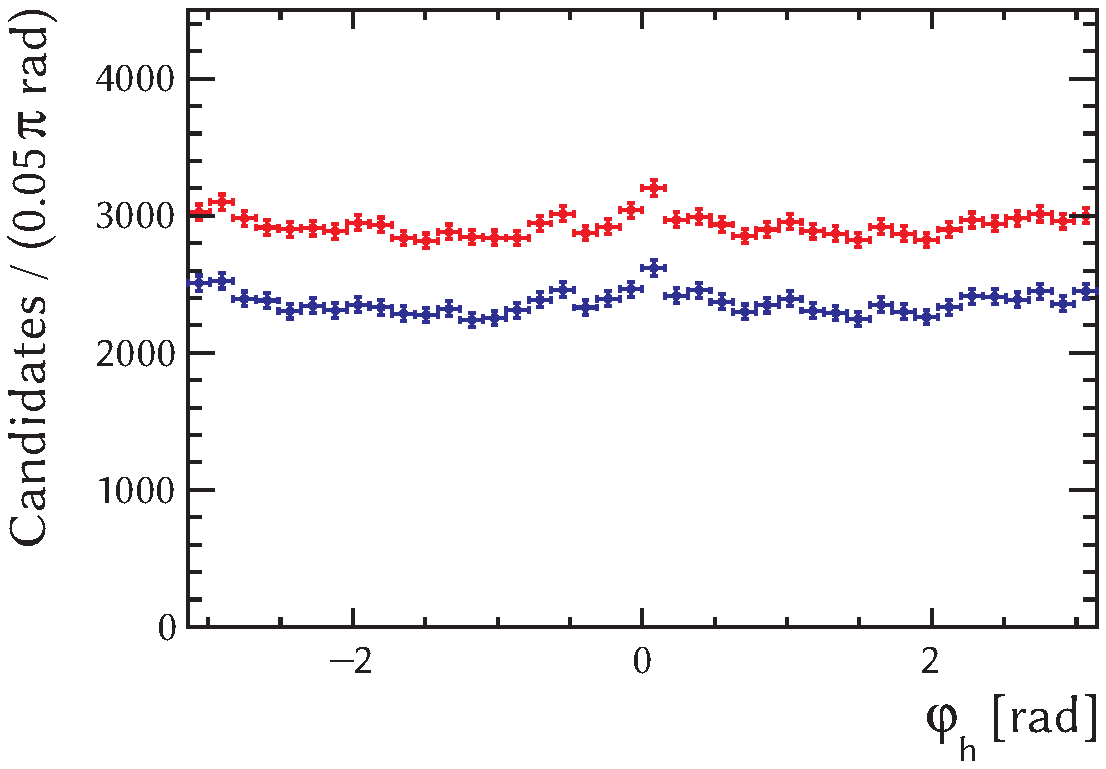
\includegraphics[width=\textwidth]{graphics/analysis/phi_bkgSub}
    \caption{}
    \label{fig:phiBkgSub}
  \end{subfigure}

  \vspace*{0.02\textwidth}
  \begin{subfigure}{0.49\textwidth}
    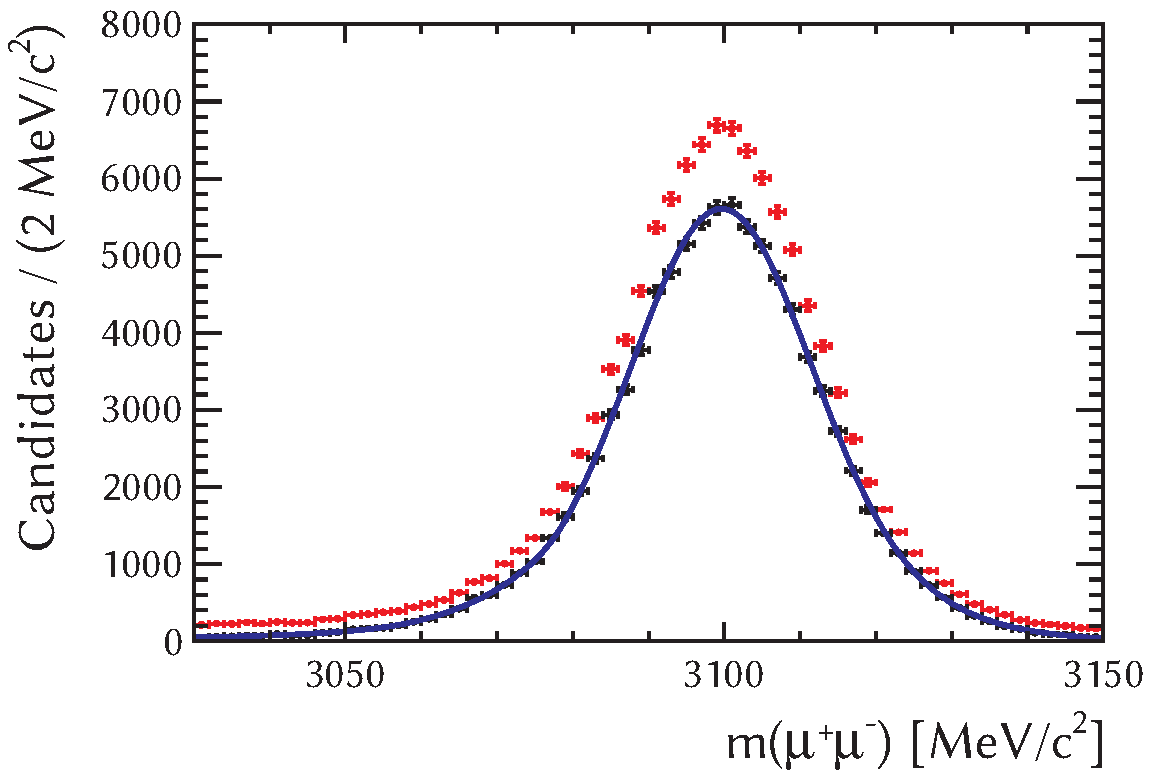
\includegraphics[width=\textwidth]{graphics/analysis/mumuMass_bkgSub_lin}
    \caption{}
    \label{fig:mumuMassBkgSub}
  \end{subfigure}%
  \hfill%
  \begin{subfigure}{0.49\textwidth}
    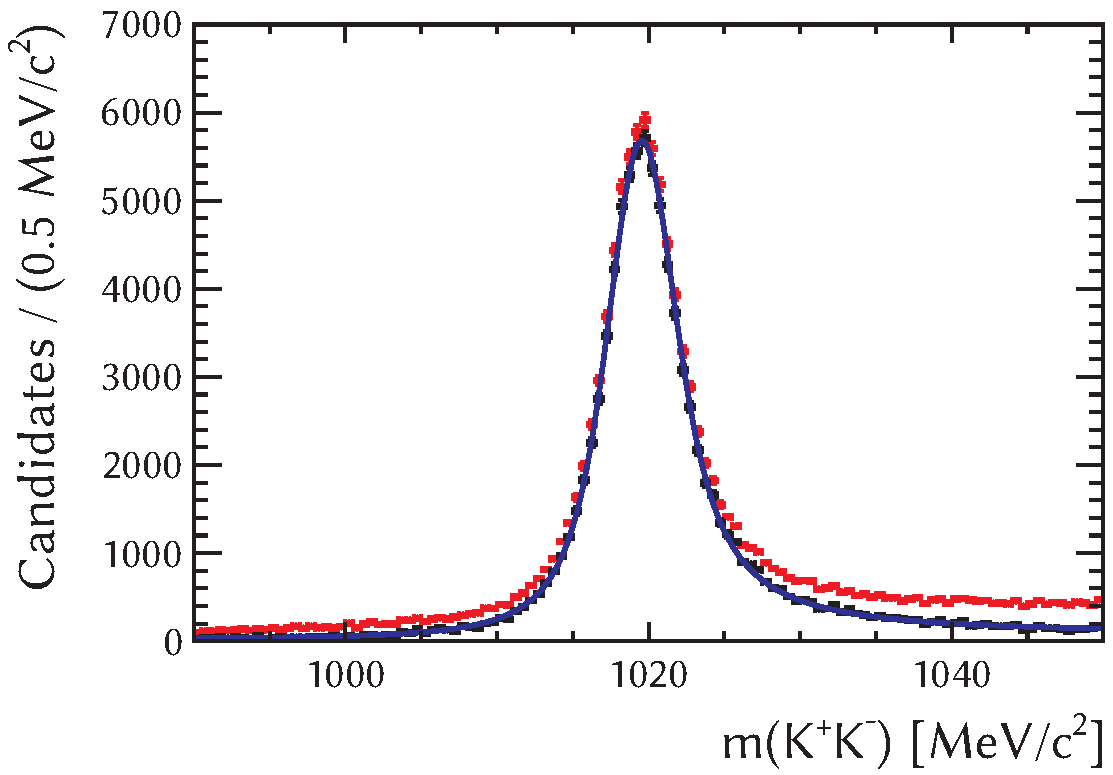
\includegraphics[width=\textwidth]{graphics/analysis/KKMass_bkgSub_lin}
    \caption{}
    \label{fig:KKMassBkgSub}
  \end{subfigure}%

  \caption{Distributions of \BstoJpsiKK{} decay candidates before (red) and after (blue) background subtraction
           in (a) decay time, (b) $\cthetaK$, (c) $\cthetal$, (d) $\phihel$, (e) $\mumu$ mass, and (f) $\KK$ mass.
           The distributions before background subtraction are for decay candidates
           in a $\JpsiKK$-mass window of 60\unitsp\MeV{} around the $\Bs$ mass.}
  \label{fig:obsBkgSub}
\end{figure}

From Figure~\ref{fig:JpsiKKMass_I2_bkgSub_ctl} it is clear that the $\JpsiKK$-mass resolution for the signal depends on the value of
$\cthetal$. This is also supported by Figure~\ref{fig:JpsiKKMassErr_ctlBins}, which shows that the distribution of the estimated
$\JpsiKK$-mass uncertainty varies for the three $\cthetal$ regions. Formally this implies that the procedure of background subtraction does
not fully work for the $\cthetal$ distribution. The impact of this effect is studied by subtracting the background with the different mass
models obtained in the $\cthetal$ intervals and a corresponding systematic uncertainty is evaluated (see Section~\ref{sec:result_syst}).

Figure~\ref{fig:obsBkgSub} shows the distributions of decay time, decay angles, $\mumu$ invariant mass, and $\KK$ invariant mass before and
after background subtraction. The distributions before background subtraction are only shown for a $\JpsiKK$-mass window of 60\unitsp\MeV{}
around the $\Bs$ mass.

From the decay-time distribution in Figure~\ref{fig:timeBkgSub} it can be seen that most background candidates have a small decay time.
Notice that the decay-time range in this plot starts at 0.3\unitsp{}ps. Even though the first of the oscillations in the decay time
distribution of the signal is lost, this requirement improves the measurement, because it removes a significant amount of background, as
shown in Section~\ref{subsec:ana_bkgSub_sel}.

The model that was fitted to the $\mumu$-mass distribution in Figure~\ref{fig:mumuMassBkgSub} consists of the sum of two Gaussian shapes,
with a polynomial that describes the enhanced tail on the left of the mass peak, which is due to photon radiation after the decay of the
$\Jpsi$. The model for the $\KK$-mass distribution consists of a relativistic Breit-Wigner shape for the $\Jpsiphi$ contribution and a
polynomial for the $\KK$ S-wave. From this fit, an S-wave fraction of approximately 5\% is found.

Note that the models for the $\mumu$ and $\KK$ mass that were used to fit the distributions in Figures~\ref{fig:mumuMassBkgSub} and
\ref{fig:KKMassBkgSub} are not used in the decay model, except for the latter in the calculation of the $\CSP$ factors (see
Section~\ref{sec:ana_KKIntegrals}). The distributions of time and angles in Figures~\ref{fig:timeBkgSub}--d are described by the model
discussed in Chapter~\ref{chap:pheno} with the experimental effects that will be discussed in the following sections.
